% -*- program: xelatex -*-

\newif\ifanswers
%\answerstrue

\documentclass[11pt]{article}

\usepackage{amssymb,amsmath,amsfonts,amsthm,graphicx}
\usepackage[top=0.3in, bottom=0.75in, left=0.5in, right=0.5in]{geometry}
\usepackage{tikz}
\usepackage{array}
\usepackage{enumitem}

\DeclareGraphicsExtensions{.pdf}

\usepackage{fontspec,realscripts}
\defaultfontfeatures{Ligatures=TeX}
\frenchspacing

\usepackage{xcolor}
\usepackage{pagecolor}
\usepackage[document]{ragged2e}

\begin{document}

\noindent
\begin{tabular*}{\textwidth}{@{\extracolsep{\fill}} l r}
\textbf{CS 310: NP-Hardness and Reductions Worksheet}
& \emph{Mudassir Shabbir, April 27, 2026}
\end{tabular*}

\vspace{0.4cm}

\noindent
\begin{tabular*}{\textwidth}{@{\extracolsep{\fill}} l l}
\textbf{Student ID 1 \& 2:}{\em (Do this in pairs)} \hrulefill
&
\end{tabular*}

\vspace{0.3cm}
\hrule

\vspace{0.4cm}

% \noindent
% \textbf{Problem Definitions.}

% \vspace{0.2cm}

% \noindent
% \textbf{3SAT:} Given a Boolean formula $\phi$ in 3-CNF (each clause has exactly three literals), decide whether there is a truth assignment to the variables that satisfies $\phi$.

% \vspace{0.2cm}

% \noindent
% \textbf{Vertex Cover (VC):} Given an undirected graph $G=(V,E)$ and an integer $k$, decide whether there exists a set $S \subseteq V$ with $|S| \le k$ such that every edge $e \in E$ has at least one endpoint in $S$.

% \vspace{0.3cm}
% \hrule
% \vspace{0.3cm}

\noindent
\textbf{A Proposed Reduction from 3SAT to Vertex Cover.}

\vspace{0.2cm}

\noindent
Given a 3-CNF formula $\phi$ with variables $x_1,\ldots,x_n$ and clauses $C_1,\ldots,C_m$, construct a graph $G=(V,E)$ and integer $k$ as follows:

\begin{enumerate}[label=\arabic*.]
    \item \textbf{Variable gadgets.} For each variable $x_i$, add two nodes labeled $x_i$ and $\bar{x}_i$ connected by an edge.
    \item \textbf{Clause gadgets.} For each clause $C_j = (\ell_{j,1} \vee \ell_{j,2} \vee \ell_{j,3})$, add a single node $c_j$ and add three edges connecting $c_j$ to the literal nodes $\ell_{j,1}$, $\ell_{j,2}$, and $\ell_{j,3}$ already in the graph (from the variable gadgets).
    \item Set $k = n + m$.
\end{enumerate}

\noindent
\textbf{Claimed correctness:} $\phi$ is satisfiable if and only if $G$ has a vertex cover of size $\le k$.

% \begin{itemize}
%   \item[($\Rightarrow$)] If $\phi$ is satisfiable, let $\tau$ be a satisfying assignment. For each $i$, place the true literal under $\tau$ (i.e., $x_i$ if $\tau(x_i)=\mathrm{T}$, or $\bar{x}_i$ if $\tau(x_i)=\mathrm{F}$) into $S$. For each clause $C_j$, place $c_j$ into $S$. Then $|S|=n+m=k$, every variable edge is covered by its true literal, and every edge incident to $c_j$ is covered by $c_j$.
%   \item[($\Leftarrow$)] If $G$ has a vertex cover $S$ with $|S| \le k = n+m$, then since each variable edge $(x_i,\bar{x}_i)$ must be covered, $S$ contains at least one of $\{x_i,\bar{x}_i\}$ for each $i$. Since $|S| \le n+m$, at most $m$ further nodes remain in $S$ to cover the clause edges. Set $\tau(x_i)=\mathrm{T}$ if $x_i \in S$, otherwise $\tau(x_i)=\mathrm{F}$. This assignment satisfies every clause because each clause edge must be covered.
% \end{itemize}

\pagenumbering{gobble}

\begin{enumerate}[leftmargin=0pt, itemindent=1.7em, itemsep=1.2em]

% -----------------------------------------------------------------------
\item \textbf{Construct the VC instance.}

Consider the following 3-CNF formula over variables $x_1, x_2, x_3$:
\[
  \phi \;=\;
  (x_1 \vee x_2 \vee x_3)
  \;\wedge\;
  (\bar{x}_1 \vee x_2 \vee x_3)
  \;\wedge\;
  (x_1 \vee \bar{x}_2 \vee x_3)
  \;\wedge\;
  (\bar{x}_1 \vee \bar{x}_2 \vee \bar{x}_3).
\]

Apply the proposed reduction to $\phi$ and draw the resulting graph $G$. List all nodes and edges explicitly, and state the value of $k$.

\vspace{9.5cm}

\ifanswers
\textbf{Sample answer.}

\medskip
\noindent
\textit{Nodes:} $x_1,\bar{x}_1,x_2,\bar{x}_2,x_3,\bar{x}_3$ (variable gadgets) and $c_1,c_2,c_3,c_4$ (clause gadgets). Total: 10 nodes.

\noindent
\textit{Edges:}
\begin{itemize}
  \item Variable edges: $(x_1,\bar{x}_1),\;(x_2,\bar{x}_2),\;(x_3,\bar{x}_3)$.
  \item Clause $C_1$: $(c_1,x_1),(c_1,x_2),(c_1,x_3)$.
  \item Clause $C_2$: $(c_2,\bar{x}_1),(c_2,x_2),(c_2,x_3)$.
  \item Clause $C_3$: $(c_3,x_1),(c_3,\bar{x}_2),(c_3,x_3)$.
  \item Clause $C_4$: $(c_4,\bar{x}_1),(c_4,\bar{x}_2),(c_4,\bar{x}_3)$.
\end{itemize}

\noindent
$k = n + m = 3 + 4 = 7$.

\medskip
\begin{center}
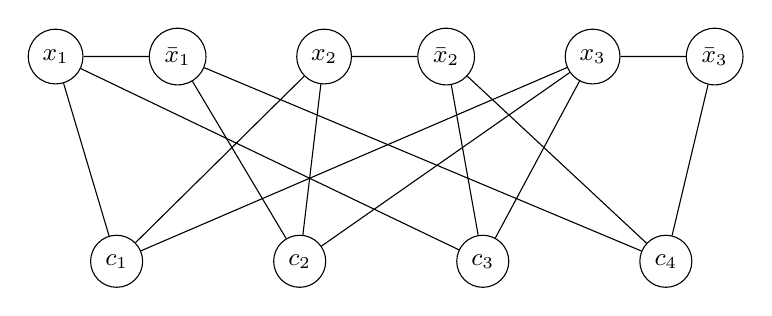
\begin{tikzpicture}[
    every node/.style={circle, draw, minimum size=0.65cm, font=\small},
    every edge/.style={draw},
    xscale=1.55, yscale=1.3
]
  % Variable gadget nodes (top row)
  \node (x1)  at (0,2)   {$x_1$};
  \node (nx1) at (1,2)   {$\bar x_1$};
  \node (x2)  at (2.2,2) {$x_2$};
  \node (nx2) at (3.2,2) {$\bar x_2$};
  \node (x3)  at (4.4,2) {$x_3$};
  \node (nx3) at (5.4,2) {$\bar x_3$};

  % Variable edges
  \draw (x1)--(nx1);
  \draw (x2)--(nx2);
  \draw (x3)--(nx3);

  % Clause nodes (bottom row)
  \node (c1) at (0.5,0)   {$c_1$};
  \node (c2) at (2.0,0)   {$c_2$};
  \node (c3) at (3.5,0)   {$c_3$};
  \node (c4) at (5.0,0)   {$c_4$};

  % C1 = (x1 v x2 v x3)
  \draw (c1)--(x1);
  \draw (c1)--(x2);
  \draw (c1)--(x3);

  % C2 = (~x1 v x2 v x3)
  \draw (c2)--(nx1);
  \draw (c2)--(x2);
  \draw (c2)--(x3);

  % C3 = (x1 v ~x2 v x3)
  \draw (c3)--(x1);
  \draw (c3)--(nx2);
  \draw (c3)--(x3);

  % C4 = (~x1 v ~x2 v ~x3)
  \draw (c4)--(nx1);
  \draw (c4)--(nx2);
  \draw (c4)--(nx3);
\end{tikzpicture}
\end{center}
\fi
\newpage
% -----------------------------------------------------------------------
\item \textbf{Verify the YES instances.}

\begin{enumerate}[label=(\alph*)]
  \item Show that $\phi$ is a YES instance of 3SAT by exhibiting a satisfying truth assignment and verifying each clause.
  \item Using the vertex cover $S$ induced by the satisfying assignment from part (a) together with all clause nodes, verify that $S$ is a valid vertex cover of size $k$ in the graph $G$ from Problem 1.
\end{enumerate}

\vspace{5.5cm}

\ifanswers
\textbf{Sample answer.}

\medskip
\noindent
\textbf{(a)} Take $x_1 = \mathrm{T},\; x_2 = \mathrm{F},\; x_3 = \mathrm{T}$.
\begin{align*}
  C_1 &= (\mathrm{T} \vee \mathrm{F} \vee \mathrm{T}) = \mathrm{T}. \\
  C_2 &= (\mathrm{F} \vee \mathrm{F} \vee \mathrm{T}) = \mathrm{T}. \\
  C_3 &= (\mathrm{T} \vee \mathrm{T} \vee \mathrm{T}) = \mathrm{T}. \quad (\bar x_2 = \mathrm{T} \text{ since } x_2=\mathrm{F})\\
  C_4 &= (\mathrm{F} \vee \mathrm{T} \vee \mathrm{F}) = \mathrm{T}. \quad (\bar x_2 = \mathrm{T})
\end{align*}
All four clauses are satisfied, so $\phi$ is a YES instance.

\medskip
\noindent
\textbf{(b)} Take $S = \{x_1,\,\bar{x}_2,\,x_3,\,c_1,\,c_2,\,c_3,\,c_4\}$. Then $|S| = 7 = k$.
\begin{itemize}
  \item Variable edges: $(x_1,\bar x_1)$ covered by $x_1$; $(x_2,\bar x_2)$ covered by $\bar x_2$; $(x_3,\bar x_3)$ covered by $x_3$.
  \item All edges incident to $c_j$ are covered because $c_j \in S$.
\end{itemize}
Every edge is covered, so $S$ is a valid vertex cover of size $k=7$.
\fi

% -----------------------------------------------------------------------
\item \textbf{Prove the reduction is incorrect.}

The reduction above contains a logical error. Identify and explain the error.

% \begin{enumerate}[label=(\alph*)]
%   \item Demonstrate that the reduction is incorrect by showing a vertex cover of size $k$ in $G$ that does \emph{not} correspond to any satisfying assignment of $\phi$. (\emph{Hint: think about what happens when you place all clause nodes in the cover.})

%   \item Identify exactly which step in the claimed ``$(\Leftarrow)$'' proof is wrong, and explain in one or two sentences why the argument breaks down.

%   \item Explain what structural change to the clause gadget would fix the reduction. You do not need to re-prove correctness; a clear description suffices.
% \end{enumerate}

\vspace{7.0cm}

\ifanswers
\textbf{Sample answer.}

\medskip
\noindent
\textbf{(a)} Consider the cover $S^* = \{x_1, x_2, x_3, c_1, c_2, c_3, c_4\}$ (all positive literals and all clause nodes), $|S^*| = 7 = k$.
\begin{itemize}
  \item Variable edges: each is covered by the positive literal endpoint.
  \item Every edge incident to any $c_j$ is covered by $c_j \in S^*$.
\end{itemize}
So $S^*$ is a valid cover of size $k$. But the assignment it encodes ($x_1=x_2=x_3=\mathrm{T}$) satisfies $\phi$ in this case. To see the real issue, note that for \emph{any} 3-CNF formula (satisfiable or not) with $n$ variables and $m$ clauses, the set consisting of \emph{any} single literal from each variable edge plus \emph{all} clause nodes has size $n + m = k$ and is always a valid vertex cover: the variable edges are covered by one endpoint, and every clause edge $(c_j, \ell)$ is covered by $c_j$. Therefore the VC instance is \emph{always} a YES instance, regardless of whether $\phi$ is satisfiable.

\medskip
\noindent
\textbf{(b)} The error is in the sentence \emph{``This assignment satisfies every clause because each clause edge must be covered.''}\ In fact, a clause edge $(c_j, \ell)$ can be covered by $c_j$ itself rather than by the literal $\ell$. When all $m$ clause nodes are in $S$, every clause edge is automatically covered, and no literal needs to be in $S$ to cover any clause edge. The proof incorrectly concludes that a covered clause edge implies a true literal in that clause.

\medskip
\noindent
\textbf{(c)} Replace each single clause node $c_j$ with a \emph{triangle} on three new nodes $u_{j,1}, u_{j,2}, u_{j,3}$ (the correct gadget from the Karp reduction). Connect each $u_{j,\ell}$ to the corresponding literal node $\ell_{j,\ell}$ in the variable gadget, and set $k = n + 2m$. A triangle requires at least 2 of its 3 nodes in any vertex cover; the connecting edges force the uncovered triangle node to correspond to a true literal, ensuring every clause is satisfied.
\fi

\end{enumerate}

\end{document}
